% -*- Mode:TeX -*-

%% IMPORTANT: The official thesis specifications are available at:
%%            http://libraries.mit.edu/archives/thesis-specs/
%%
%%            Please verify your thesis' formatting and copyright
%%            assignment before submission.  If you notice any
%%            discrepancies between these templates and the 
%%            MIT Libraries' specs, please let us know
%%            by e-mailing thesis@mit.edu

%% The documentclass options along with the pagestyle can be used to generate
%% a technical report, a draft copy, or a regular thesis.  You may need to
%% re-specify the pagestyle after you \include  cover.tex.  For more
%% information, see the first few lines of mitthesis.cls. 

%\documentclass[12pt,vi,twoside]{mitthesis}
%%
%%  If you want your thesis copyright to you instead of MIT, use the
%%  ``vi'' option, as above.
%%
%\documentclass[12pt,twoside,leftblank]{mitthesis}
%%
%% If you want blank pages before new chapters to be labelled ``This
%% Page Intentionally Left Blank'', use the ``leftblank'' option, as
%% above. 

\documentclass[12pt,twoside]{mitthesis}
\usepackage{lgrind}
%% These have been added at the request of the MIT Libraries, because
%% some PDF conversions mess up the ligatures.  -LB, 1/22/2014
\usepackage{cmap}
\usepackage[T1]{fontenc}
\pagestyle{plain}

%% This bit allows you to either specify only the files which you wish to
%% process, or `all' to process all files which you \include.
%% Krishna Sethuraman (1990).

\typein [\files]{Enter file names to process, (chap1,chap2 ...), or `all' to
process all files:}
\def\all{all}
\ifx\files\all \typeout{Including all files.} \else \typeout{Including only \files.} \includeonly{\files} \fi

\begin{document}

% -*-latex-*-
% 
% For questions, comments, concerns or complaints:
% thesis@mit.edu
% 
%
% $Log: cover.tex,v $
% Revision 1.8  2008/05/13 15:02:15  jdreed
% Degree month is June, not May.  Added note about prevdegrees.
% Arthur Smith's title updated
%
% Revision 1.7  2001/02/08 18:53:16  boojum
% changed some \newpages to \cleardoublepages
%
% Revision 1.6  1999/10/21 14:49:31  boojum
% changed comment referring to documentstyle
%
% Revision 1.5  1999/10/21 14:39:04  boojum
% *** empty log message ***
%
% Revision 1.4  1997/04/18  17:54:10  othomas
% added page numbers on abstract and cover, and made 1 abstract
% page the default rather than 2.  (anne hunter tells me this
% is the new institute standard.)
%
% Revision 1.4  1997/04/18  17:54:10  othomas
% added page numbers on abstract and cover, and made 1 abstract
% page the default rather than 2.  (anne hunter tells me this
% is the new institute standard.)
%
% Revision 1.3  93/05/17  17:06:29  starflt
% Added acknowledgements section (suggested by tompalka)
% 
% Revision 1.2  92/04/22  13:13:13  epeisach
% Fixes for 1991 course 6 requirements
% Phrase "and to grant others the right to do so" has been added to 
% permission clause
% Second copy of abstract is not counted as separate pages so numbering works
% out
% 
% Revision 1.1  92/04/22  13:08:20  epeisach

% NOTE:
% These templates make an effort to conform to the MIT Thesis specifications,
% however the specifications can change.  We recommend that you verify the
% layout of your title page with your thesis advisor and/or the MIT 
% Libraries before printing your final copy.
\title{Sieve: Provably Secure Access Control for User-Managed Storage}

\author{Frank Yi-Fei Wang}
% If you wish to list your previous degrees on the cover page, use the 
% previous degrees command:
%       \prevdegrees{A.A., Harvard University (1985)}
% You can use the \\ command to list multiple previous degrees
%       \prevdegrees{B.S., University of California (1978) \\
%                    S.M., Massachusetts Institute of Technology (1981)}
\department{Department of Electrical Engineering and Computer Science}

% If the thesis is for two degrees simultaneously, list them both
% separated by \and like this:
% \degree{Doctor of Philosophy \and Master of Science}
\degree{Master of Science}

% As of the 2007-08 academic year, valid degree months are September, 
% February, or June.  The default is June.
\degreemonth{February}
\degreeyear{2016}
\thesisdate{January 29, 2016}

%% By default, the thesis will be copyrighted to MIT.  If you need to copyright
%% the thesis to yourself, just specify the `vi' documentclass option.  If for
%% some reason you want to exactly specify the copyright notice text, you can
%% use the \copyrightnoticetext command.  
%\copyrightnoticetext{\copyright IBM, 1990.  Do not open till Xmas.}

% If there is more than one supervisor, use the \supervisor command
% once for each.
\supervisor{Nickolai Zeldovich}{Associate Professor}

% This is the department committee chairman, not the thesis committee
% chairman.  You should replace this with your Department's Committee
% Chairman.
\chairman{Professor Leslie A. Kolodziejski}{Chairman, Department Committee on Graduate Theses}

% Make the titlepage based on the above information.  If you need
% something special and can't use the standard form, you can specify
% the exact text of the titlepage yourself.  Put it in a titlepage
% environment and leave blank lines where you want vertical space.
% The spaces will be adjusted to fill the entire page.  The dotted
% lines for the signatures are made with the \signature command.
\maketitle

% The abstractpage environment sets up everything on the page except
% the text itself.  The title and other header material are put at the
% top of the page, and the supervisors are listed at the bottom.  A
% new page is begun both before and after.  Of course, an abstract may
% be more than one page itself.  If you need more control over the
% format of the page, you can use the abstract environment, which puts
% the word "Abstract" at the beginning and single spaces its text.

%% You can either \input (*not* \include) your abstract file, or you can put
%% the text of the abstract directly between the \begin{abstractpage} and
%% \end{abstractpage} commands.

% First copy: start a new page, and save the page number.
\cleardoublepage
% Uncomment the next line if you do NOT want a page number on your
% abstract and acknowledgments pages.
% \pagestyle{empty}
\setcounter{savepage}{\thepage}
\begin{abstractpage}
% $Log: abstract.tex,v $
% Revision 1.1  93/05/14  14:56:25  starflt
% Initial revision
% 
% Revision 1.1  90/05/04  10:41:01  lwvanels
% Initial revision
% 
%
%% The text of your abstract and nothing else (other than comments) goes here.
%% It will be single-spaced and the rest of the text that is supposed to go on
%% the abstract page will be generated by the abstractpage environment.  This
%% file should be \input (not \include 'd) from cover.tex.
In today's web, applications whose
value depends on access to user
data, such as quantified self applications
and applications that analyze medical
records, suffer when user data is 
locked in application servers.
In this thesis, we present Sieve,
a new system that solves
this problem by centralizing
user data. It provides
secure, delegated access to a user's
sensitive cloud data. Sieve enforces
\emph{cryptographically strong
restrictions} on how third party
web services can access that data.
However, Sieve can still be compatible
with monetization systems like targeted
advertising, reducing the barrier to
adoption. In Sieve, each user uploads
her data in encrypted form to a
cloud-based storage provider. 

Each data object is associated with
attributes like file type, subject
matter, and associated user names;
these attributes arise from automatic
annotation or manual user tagging.
When a web service requests access
to the user's data, she generates
a service-specific access policy.
This policy is expressed in terms of
attributes and simple operators like
equals and less-than. Using attribute-based
encryption, Sieve automatically translates
the human-readable access policy into a
public/private key pair that is given
to the web service. The key pair allows
the web service to independently access
and decrypt the delegated user objects
(but no others). Unlike other systems
that use attribute based encryption,
Sieve provides strong revocation semantics
and distributed trust. Using this scheme,
Sieve provides users with true control
over how their cloud data is accessed.
This contrasts with popular delegation
schemes like OAuth in which policies
are written by web services and lacking
in cryptographically strong protections.

\end{abstractpage}

% Additional copy: start a new page, and reset the page number.  This way,
% the second copy of the abstract is not counted as separate pages.
% Uncomment the next 6 lines if you need two copies of the abstract
% page.
% \setcounter{page}{\thesavepage}
% \begin{abstractpage}
% % $Log: abstract.tex,v $
% Revision 1.1  93/05/14  14:56:25  starflt
% Initial revision
% 
% Revision 1.1  90/05/04  10:41:01  lwvanels
% Initial revision
% 
%
%% The text of your abstract and nothing else (other than comments) goes here.
%% It will be single-spaced and the rest of the text that is supposed to go on
%% the abstract page will be generated by the abstractpage environment.  This
%% file should be \input (not \include 'd) from cover.tex.
In today's web, applications whose
value depends on access to user
data, such as quantified self applications
and applications that analyze medical
records, suffer when user data is 
locked in application servers.
In this thesis, we present Sieve,
a new system that solves
this problem by centralizing
user data. It provides
secure, delegated access to a user's
sensitive cloud data. Sieve enforces
\emph{cryptographically strong
restrictions} on how third party
web services can access that data.
However, Sieve can still be compatible
with monetization systems like targeted
advertising, reducing the barrier to
adoption. In Sieve, each user uploads
her data in encrypted form to a
cloud-based storage provider. 

Each data object is associated with
attributes like file type, subject
matter, and associated user names;
these attributes arise from automatic
annotation or manual user tagging.
When a web service requests access
to the user's data, she generates
a service-specific access policy.
This policy is expressed in terms of
attributes and simple operators like
equals and less-than. Using attribute-based
encryption, Sieve automatically translates
the human-readable access policy into a
public/private key pair that is given
to the web service. The key pair allows
the web service to independently access
and decrypt the delegated user objects
(but no others). Unlike other systems
that use attribute based encryption,
Sieve provides strong revocation semantics
and distributed trust. Using this scheme,
Sieve provides users with true control
over how their cloud data is accessed.
This contrasts with popular delegation
schemes like OAuth in which policies
are written by web services and lacking
in cryptographically strong protections.

% \end{abstractpage}

\cleardoublepage

\section*{Acknowledgments}

I am indebted to my advisor, Nickolai Zeldovich, for helping me with all
aspects of this project from its inception to its publication at NSDI 2016.
I am also extremely thankful to my collaborator and one of the funniest
man I know, James Mickens, for his valuable mentorship. 
He was an important part of this project and helped with much of the writing. 

I would also like to thank everyone who has contributed and provided valuable
feedback along the way, including Vinod Vaikuntanathan, Peter Bailis, Engin Kirda,
Wil Robertson, and the Recursers. I would like to thank everyone who have provided
me support and made my research experience awesome. Specifically, I would like to
thank Ravi Netravali, Jen Gong, Amy Zhao, Nora Ou, Amy Ousterhout, David Lazar,
the rest of the PDOS lab, and my friends at MIT and Sidney-Pacific.

I would also like to thank NSF Graduate Fellowship and Jacobs Presidential Fellowship
for providing me with financial support to conduct this research. 

Finally, I would like to thank my family who has supported my decision
to move to the other side of the country to pursue my PhD and have provided support
in many forms from the west coast. This work would not have been possible
without their continued support.
%%%%%%%%%%%%%%%%%%%%%%%%%%%%%%%%%%%%%%%%%%%%%%%%%%%%%%%%%%%%%%%%%%%%%%
% -*-latex-*-

% Some departments (e.g. 5) require an additional signature page.  See
% signature.tex for more information and uncomment the following line if
% applicable.
% % -*- Mode:TeX -*-
%
% Some departments (e.g. Chemistry) require an additional cover page
% with signatures of the thesis committee.  Please check with your
% thesis advisor or other appropriate person to determine if such a 
% page is required for your thesis.  
%
% If you choose not to use the "titlepage" environment, a \newpage
% commands, and several \vspace{\fill} commands may be necessary to
% achieve the required spacing.  The \signature command is defined in
% the "mitthesis" class
%
% The following sample appears courtesy of Ben Kaduk <kaduk@mit.edu> and
% was used in his June 2012 doctoral thesis in Chemistry. 

\begin{titlepage}
\begin{large}
This doctoral thesis has been examined by a Committee of the Department
of Chemistry as follows:

\signature{Professor Jianshu Cao}{Chairman, Thesis Committee \\
   Professor of Chemistry}

\signature{Professor Troy Van Voorhis}{Thesis Supervisor \\
   Associate Professor of Chemistry}

\signature{Professor Robert W. Field}{Member, Thesis Committee \\
   Haslam and Dewey Professor of Chemistry}
\end{large}
\end{titlepage}


\pagestyle{plain}
  % -*- Mode:TeX -*-
%% This file simply contains the commands that actually generate the table of
%% contents and lists of figures and tables.  You can omit any or all of
%% these files by simply taking out the appropriate command.  For more
%% information on these files, see appendix C.3.3 of the LaTeX manual. 
\tableofcontents
\newpage
\listoffigures
\newpage
\listoftables


%% This is an example first chapter.  You should put chapter/appendix that you
%% write into a separate file, and add a line \include{yourfilename} to
%% main.tex, where `yourfilename.tex' is the name of the chapter/appendix file.
%% You can process specific files by typing their names in at the 
%% \files=
%% prompt when you run the file main.tex through LaTeX.
\chapter{Introduction}

In today's web, a single person often 
uses multiple web services. 
Conceptually, the user has a single
logical data set, and she selectively
exposes a portion of that data to each
web service. In practice, the services
control her data: each service keeps its
portion of the user's objects in a walled
garden which neither the user nor external
services can directly access.

These service-controlled data silos force
users to relinquish low-level authority over
data storage. As a result, users cede the
ultimate power to set access controls and
limit how their data is shared. Furthermore, simple
operations like enumerating all of a user's
cloud data become difficult, since a user's
state is scattered across a variety of services
which hide raw storage via high-level, curated
APIs.

Data silos are not only problematic for
users but also problematic for
\emph{applications} whose value often scales
with the amount of user data that can be
accessed by the application. For example,
quantified self applications~\cite{beam},
which track a user's health and personal
productivity, work best when given data
from a variety of sensors and environmental
locations. Similarly, applications which analyze a
user's medical records~\cite{lark} or financial
transactions~\cite{mint} produce the best
results when they have access to 
all of the user's medical or financial data.
Unfortunately, modern web services use
a siloed design that limits a user's ability to share 
data outside of the service-specific silo. 
For example, wearable
fitness-tracking sensors typically upload data
to vendor-specific cloud storage, and medical
records are often bound to storage that belongs
to the medical specialist who measured the
data. Thus, having a user-centric storage model
is beneficial for \emph{both} the user and the application.
However, using such a model poses new challenges.
In the next section, we describe these main challenges.

\section{The Challenges of Centralized Data}

In a user-centric storage model, a user's
entire data set would reside in a single,
logically centralized cloud store; the user
would selectively disclose portions of that
data to individual third party applications.
Systems like Amber~\cite{amber} and BStore~\cite{bstore}
have demonstrated the benefits of 
decoupling applications and user
data, but a centralized data storage
increases the damage that results from a
subverted or curious storage provider because
\emph{all} of a user's cleartext data is at
risk, instead of a service-specific subset.

To protect against untrusted storage providers,
users can encrypt data before uploading it.
However, the ultimate purpose of uploading
data is to share it with third party services.
Thus, users need a way to selectively expose
pointers to encrypted objects (and the associated
decryption keys). Protocols exist for sharing
cloud data across multiple services, but these
protocols have major usability and security
problems. For example, the popular OAuth
protocol~\cite{oauth} enables cross-site data
sharing via delegated API calls (i.e., API
calls that act with the authority of a user).
However, OAuth policies are invariably defined
by web services, not by users. Furthermore,
OAuth does not enforce cryptographically strong
constraints on the data that the delegated
APIs can access. Thus, even if a user could
generate her own OAuth policies, she would
lack strong assurances about what those policies
mean, and how they are enforced.

Given the discussion above, logically centralized
storage seems good for users in theory, but
difficult to implement in practice. In this
paper, we address three specific challenges
that emerge from a logically centralized storage
architecture. The first is \emph{security}: how
do we make access controls cryptographically
strong, and protect user data against the
compromise of storage providers and user devices?
The second challenge is \emph{usability}: how
can we express access policies in a way that
lay-person users will understand, but is
translatable to cryptographically enforceable
mechanisms? The final challenge is \emph{application
richness}: after we have moved user data out
of per-application silos and into user-controlled
storage, how can we support the complex 
applications that users currently enjoy?

\begin{figure}
  \centering
     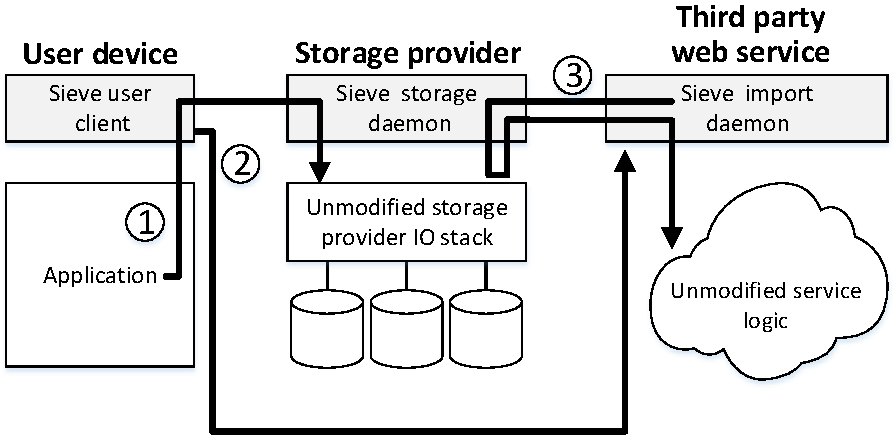
\includegraphics{figs/arch.pdf}
     \caption[Sieve's high-level architecture]
     {Sieve's high-level architecture. 1) The user uploads
              ABE-encrypted data to a storage provider. 2) The user
              generates a data policy for a third party web
              service. Sieve translates the policy into an ABE
              decryption key, and sends the key to the web service.
              3) The web service pulls encrypted data from the
              storage provider, decrypts it locally, and injects
              the data into the unmodified application pipeline.}
  \label{fig:sieve}
\end{figure}

\section{Our Solution}

To address these challenges, we propose Sieve,
a new system for delegating access to
private cloud data. Figure~\ref{fig:sieve} depicts
Sieve's high-level workflow. A user generates
raw data on her computational devices, and
uploads encrypted versions of it to a single cloud
repository; the user manages and pays for the 
cloud, not the web services which
desire access to the data. When a third party web service
requests access, e.g., during the first
time that a user visits a site, the user
generates a high-level access policy (\S\ref{sec:policies})
for the service. Sieve splits the policy into
two pieces: the storage provider learns which
objects a third party can access (but not the
cleartext versions of those objects), and the
third party learns the objects that it can
access, and the corresponding decryption keys,
while learning nothing about the rest of the
user's data set. Once the third party has
downloaded the necessary objects and decrypted
them, it feeds the cleartext data to a legacy
pipeline for processing user content (\S\ref{sec:attrGen}).

\begin{figure}
\centering
\begin{verbatim}
              (type="Fitness" OR type="Medical") AND (date > 2012) 
                              AND (source="FitBit") 
\end{verbatim}
\caption[Example Sieve policy]{Example Sieve policy for an exercise application.}
\label{fig:policyex}
\end{figure}

Sieve leverages three techniques to implement
the workflow in Figure~\ref{fig:sieve}:\\
\begin{smitemize}
  \item Sieve uses \textbf{attribute-based encryption}
  (ABE)~\cite{kpabe} to implement cryptographically strong access
  policies. In ABE, encrypted data is 
  associated with attributes, which are key-value 
  pairs like ``date=2012", and decryption keys are 
  associated with policies; a key can only
  decrypt ciphertexts whose attributes satisfy a key's
  policy. Before the user uploads
  objects to the storage provider, she (or her local
  device) tags the objects with attributes like the
  date, the user's current location, or the object type
  (e.g., ``medical'', ``financial'', ``fitness").
  The uploading device transparently encrypts the objects
  with the relevant attributes before sending the objects to
  the storage provider. Later, when a third party web service 
  requests access to the user's data, the user creates a policy
  defined in terms of attributes and attribute
  operators like equality and less than. Figure~\ref{fig:policyex}
  shows an example of such a policy, which a user
  might give an application that visualizes her exercise data.
  The user's local device automatically translates the
  policy into an ABE decryption key, and sends the key
  to the web service. Afterwards, the web service can use
  the key to read the cleartext versions of the delegated
  objects from the storage provider and does not require
  any more communication with the user.
  
  \item To revoke a third party's access to sensitive data,
  the user informs the storage provider that the third
  party should no longer be able to download encrypted
  user objects. However, the third party still possesses
  the associated decryption key, and can decrypt leaked
  ciphertext if the storage server is later compromised.
  To prevent this scenario, Sieve uses \textbf{key
  homomorphism}~\cite{keyhom} to implement key revocation. Key
  homomorphism allows the storage provider
  to re-encrypt user data without learning the underlying
  cleartext--the storage provider merely reads the
  ciphertext and writes the output of a function that
  accepts the ciphertext and a user-specified rekeying
  token as input. The execution of this function on the storage 
  provider also does not reveal any information about the 
  cleartext data. Using \textit{in situ} re-encryption,
  users can avoid re-encrypting data on user devices and
  then re-uploading it. Additionally, if storage providers
  are honest at the time of key revocation, subsequent
  storage provider compromises will not reveal data that
  is encrypted with keys that are revoked (but possibly
  still in the wild). To our knowledge, Sieve is the first 
  ABE-based system to support full re-keying of \textit{both}
  the metadata and data.

  \item ABE uses a \emph{master secret key} to generate
  decryption keys. The loss of this key results
  in the compromise of the entire cryptosystem. In
  standard ABE schemes, the master secret is kept by a
  single trusted authority. In the context of Sieve,
  this would mean keeping the master secret on a single
  user device. This is unattractive, since user devices
  are often lost or stolen. Thus, Sieve
  uses \textbf{secret-sharing} and \textbf{two-factor
  authentication} to partition the master secret across
  multiple devices, and prevent unauthorized devices
  from arbitrarily participating in Sieve's cryptographic
  protocols.
    
\end{smitemize}

Sieve represents a middle ground between today's
popular web services (which provide weak user
control over the distribution and access of her data), 
and proposed systems from the
research community which strengthen user control,
but greatly restrict server-side computation~\cite{mylar}
or eliminate it altogether~\cite{sundr,depot,sporc,bstore,depSky}.
Sieve explores a
different point in the design space, one that
provides cryptographically strong access controls
to users while still permitting the rich
server-side computation on user's sensitive data
that many popular web
applications require to provide increased value
for the user.

To demonstrate its practicality, we integrated Sieve with
an existing health application, Open mHealth~\cite{omh},
an open-source application that 
helps users store and visualize their data. We obtained
realistic user health data based on existing clinical standards
from Open mHealth and used Sieve 
to manage the user data (\S\ref{sec:integration}).

\chapter{Threat Model and Security Goals}
\label{sec:threatModel}

We focus on three kinds of principals. A
\textbf{user} is someone who wants to store
data online and selectively expose it
to a \textbf{third party web service}. The
user stores her (encrypted) data on a
\textbf{cloud storage provider}. Each
user has one storage provider, but
potentially many third parties which
need delegated access. We envision storage
providers be operated by services 
such as Amazon S3 and Microsoft
Azure. Potential third party web services
are FitBit, Lark, Misfit, Mint, and 
any other application that generates new value
from sensitive user data.

\section{Threat Model}
Sieve protects against a curious cloud
provider or external attacker from
gaining access to user data stored
on the cloud storage provider. We assume
the attacker is \textit{passive}, meaning
they can access the data but do not interfere
in any Sieve protocols. 

Sieve prevents the web service from trying
to access more data than allowed by its
access policies. Moreover, Sieve allows for full revocation
of a web service's data access:
after revocation, the web service cannot
access any previously retrievable data
even if the storage provider is compromised.

The user is trusted, but Sieve assumes that
the user might lose devices. Sieve
provides a way to recover from device 
losses, but Sieve does not protect against
a subverted device that the user believes 
is functioning properly, i.e. a device
installed with a rootkit.

Sieve does not protect against client-side
attacks like social engineering~\cite{socialEngineering}
or cross-site scripting~\cite{xss}.

\section{Security Goals}
The user has a financial agreement with
the storage provider: the user pays for the provider 
to keep her objects and to participate in the
Sieve protocol on her behalf.
The user places encrypted data on the
storage provider, but never reveals
the decryption keys to the provider. 
This protects the confidentiality of
user data if the storage service is
malicious or compromised. Using signatures,
Sieve protects the data's
integrity. However, Sieve cannot
guarantee the availability or freshness
of the data that the storage provider
delivers to a web service. If desired,
Sieve can be layered atop storage
systems like CloudProof~\cite{cloudproof}
which do provide those properties.

Sieve does not hide access patterns
or object metadata (i.e., attributes) from
the storage provider. Thus, a curious
provider can learn which encrypted
objects a third party has been authorized
to read, as well as the attributes
that are associated with those objects.
If users are concerned about data
leakage via access patterns, they
could layer Sieve atop an ORAM
protocol~\cite{shroud}. To hide attributes,
Sieve could also use predicate encryption~\cite{katz2008,shen2009}.
However, ORAM and predicate encryption
incur heavy performance overheads
(\S\ref{sec:related}), so Sieve uses
lighter weight mechanisms that reduce
service latency at the cost of leaking
more metadata. We believe that this
trade-off is reasonable for many users
and companies, given the importance
of low latencies in modern web services~\cite{wprof,bobtail}.

With respect to third party web services,
Sieve's goal is to reveal user data only
as permitted by the user's disclosure
policies. After Sieve transmits information
to a third party web server, Sieve cannot
restrict what the third party does with that
data, since third parties may cache user data
locally, even after the user has revoked access
to the canonical versions that reside on her
storage server. Third parties can also share 
decrypted user data with other
principals via out-of-band, non-Sieve protocols
like in the current web infrastructure.
Solving these issues is beyond the scope of
this paper. However, if a web service shares its user-issued
ABE key, Sieve can revoke it, preventing
those parties from downloading old or new
user data from the storage provider
(\S\ref{sec:revocation}).

Sieve uses secret sharing to
protect system-wide secrets like the ABE
master key from the loss of a single device
(\S\ref{sec:secretSharing}).

\appendix
\chapter{Tables}

\begin{table}
\caption{Armadillos}
\label{arm:table}
\begin{center}
\begin{tabular}{||l|l||}\hline
Armadillos & are \\\hline
our	   & friends \\\hline
\end{tabular}
\end{center}
\end{table}

\clearpage
\newpage

\chapter{Figures}

\vspace*{-3in}

\begin{figure}
\vspace{2.4in}
\caption{Armadillo slaying lawyer.}
\label{arm:fig1}
\end{figure}
\clearpage
\newpage

\begin{figure}
\vspace{2.4in}
\caption{Armadillo eradicating national debt.}
\label{arm:fig2}
\end{figure}
\clearpage
\newpage

%% This defines the bibliography file (main.bib) and the bibliography style.
%% If you want to create a bibliography file by hand, change the contents of
%% this file to a `thebibliography' environment.  For more information 
%% see section 4.3 of the LaTeX manual.
\begin{singlespace}
\bibliography{main}
\bibliographystyle{plain}
\end{singlespace}

\end{document}

